\chapter{Duality in deep learning}
\label{sec:duality}

\section{Old optimizer, new norm}
\label{subsec:old-optimizer-new-norm}

\textit{Contribution statement: The ideas in this section are primarily due to Jeremy Bernstein. The narrative adapts two papers we wrote together, ``Old Optimizer, New Norm: An Anthology'' and ``Modular Duality in Deep Learning'' \citep{bernstein2024anthology,bernstein2024duality}.}

\vspace{1em}

This section tells the story of how three popular optimizers---SGD, Adam, and Shampoo---can each be understood from a common concept called \textit{duality}. The upshot is that the first step of metrizing deep learning---equipping activation spaces with \textit{norms}---links past optimizers under a common framework and may provide inspiration for designing faster, more scalable optimizers. The section after this one will show how duality leads to the Muon optimizer, which set speed records for training NanoGPT \citep{modded_nanogpt_2024} and has since been validated at scale \citep{liu2025muonscalablellmtraining,shah2025muonpretraining}.

The spirit of duality is that an ideal optimizer wants two things at once:
\begin{enumerate}
    \item Reduce the loss the most.
    \item Disturb the model the least.
\end{enumerate}
But to reduce the loss, the model must change. The compromise is constrained optimization:
\begin{equation}
    \argmin_{\Delta W} \; \trace(G^\top \Delta W) \; \text{ such that } \; \norm{\Delta W} \leq \eta,
\end{equation} where $G$ is the gradient, $\Delta W$ is the weight update, and $\trace(G^\top \Delta W)$ is the linearized improvement in the loss. A question arises: how to measure the size of the disturbance $\Delta W$? This question is at the heart of duality. Different optimizers make different choices, summarized in \cref{tab:weight_update_rules}. This section tells the story of three such choices. Credit to Jianlin Su for putting the spirit of duality in these terms \citep{kexuefm-10739}.

\renewcommand{\arraystretch}{1.5}
\begin{table}[t]
    \centering
    \begin{tabular}{ccccc}
        \toprule
        \textbf{Domain} & \textbf{Norm} & \hspace{1.3em}\textbf{Duality Map} & \textbf{Optimizer} & \textbf{Cousin}\\
        \midrule
        $\R^n$ & Euclidean $\ell_2$ & $\displaystyle g \mapsto  \tfrac{g}{\norm{g}_2}$ & gradient descent & SGD \\
        
        $\R^n$ & infinity $\ell_\infty$ & $\displaystyle g \mapsto \sign(g)$ & sign descent & Adam \\
        
        $\R^{m\times n}$ & spectral $\ell_{2\to2}$ & $\displaystyle G \mapsto UV^\top$ & spectral descent & Shampoo, Muon \\
        \bottomrule
    \end{tabular}
    \caption{Popular optimizers are related to duality maps under different norms. In spectral descent, the gradient is viewed as a matrix. Its singular value decomposition is $G = U \Sigma V^\top$.}
    \label{tab:weight_update_rules}
\end{table}
\renewcommand{\arraystretch}{1}

One motivation behind duality is that there is a type mismatch in the most basic form of gradient descent. To pass the type check, the gradient must be passed through a \textit{duality map} before being multiplied by the learning rate and subtracted:

\begin{center}
    \begin{minipage}{0.6\textwidth}
    $\mathtt{weight} - \mathtt{LR}\,\mathtt{*}\,\mathtt{weight.grad}$ \hfill \texttt{\textcolor{BrickRed}{type error!}} \\
    $\mathtt{weight} - \mathtt{LR}\,\mathtt{*}\,\mathtt{dualize}(\mathtt{weight.grad})$ \hfill \texttt{\textcolor{ForestGreen}{all good!}}
    \end{minipage}
\end{center}

The reason is that a gradient is a \textit{dual} vector, an entirely different object from a weight. The difference is well understood in physics, where Professor Netta Engelhardt at MIT once opened a general relativity lecture by asking, ``How many of you have been lied to that the gradient is a vector?'' It is also understood in mirror descent \citep{nemirovsky_yudin_1983}, natural gradient descent \citep{amari2016information}, and steepest descent under a norm \citep{boyd2004convex}. A duality map must first map the gradient to the primal space.

\begin{definitionbox}[Dual vector, dual space, and duality map]
    Given a vector space $V$, a \textit{dual vector} is any linear function $f : V \to \R$. For example, row vectors are functions that map column vectors to real numbers via a dot product. The \textit{dual space} $V^\ast$ of $V$ is the set of dual vectors on $V$. The dual space is itself a vector space, with addition defined $(f + g)(x) = f(x) + g(x)$ and scalar multiplication defined $(\alpha f)(x) = \alpha f(x)$. A \textit{duality map} is any function that sends a member of the dual space $V^\ast$ to a member of the primal space $V$. We do not require that applying a duality map twice must equal the identity map. Given a dual vector $f \in V^\ast$, its functional form $f(\cdot)$ is often written as an inner product $\langle f, \cdot \rangle$, which is possible by the Riesz representation theorem \citep{Riesz1907}.
\end{definitionbox}

Why is the gradient a dual vector? Let $\el : \mathcal{W} \to \R$ denote a differentiable loss function for a machine learning model with weight space $\mathcal{W}$. The gradient is a dual vector because, in the Taylor expansion of the loss, \begin{equation}\label{eq:taylor}
    \el(W+\Delta W) = \el(W) + \langle \nabla_W\el(W), \Delta W \rangle + \text{higher-order terms},
\end{equation}
the gradient appears as a function $\langle \nabla_W \el(W), \cdot \rangle$. This function takes in a weight perturbation $\Delta W$ and outputs a real number representing the linearized change in loss due to the weight perturbation. Therefore the gradient lives in a different vector space from the weights. A priori, there is no clear way to add the two.

The weight space may well be $\R^{m \times n}$, and the gradient may well be the exact same shape. But enforcing the restriction not to add them is a reminder that the loss function may have highly heterogenous curvature. The raw gradient might not respect this heterogeneity, unless a good duality map corrects the size and direction of the gradient to better attune it to the curvature in the loss function.

One path to arrive at duality is steepest descent under a norm. As in \cref{sec:intro}, suppose that there is some norm $\norm{\cdot} : \mathcal{W} \to \R$ and sharpness parameter $\lambda > 0$ that serve as a good local approximation of the loss, \begin{equation}
    \el(W+\Delta W) \approx \el(W) + \langle \nabla_W\el(W), \Delta W \rangle + \frac{\lambda}{2} \cdot \norm{\Delta W}^2.
\end{equation} If this approximation is good, a weight update should find a $\Delta W$ to minimize it. The solution splits into a \textit{step size} based on a dual norm and a \textit{step direction} based on a duality map.

\begin{definitionbox}[Dual norm and duality map based on a norm]
    \label{def:dual-norm-and-duality-map}
    Given a norm $\norm{\cdot}:V\to\R$ on a vector space $V$, the \textit{dual norm} $\norm{\cdot}^\dagger$ of a dual vector $G \in V^\ast$ is
    \begin{equation*}
    \norm{G}^\dagger \defeq \max_{T\in V:\norm{T}=1} \, \langle G, T \rangle.
    \end{equation*}
    The \textit{duality map based on a norm} is
    \begin{equation*}
    \dualize_{\norm{\cdot}} G \defeq \argmax_{T\in V:\norm{T}=1} \, \langle G, T \rangle,
    \end{equation*}
    where, if the $\argmax$ is not unique, $\dualize_{\norm{\cdot}}$ returns any maximizer.
\end{definitionbox}

\begin{theorembox}[Steepest descent under a norm]
    \label{theorem:steepest}
    For any dual vector $G \in V^\ast$ thought of as ``the gradient,'' any sharpness $\lambda \geq 0$, and any norm $\norm{\cdot}: V \to \R$ with dual norm $\norm{\cdot}^\dagger$ and duality map $\dualize_{\norm{\cdot}}$, steepest descent splits into a step size based on the dual norm and a step direction based on the duality map:
\begin{gather*}\label{eq:dual-steepest}
    \argmin_{\Delta W \in V} \left[ \langle G, \Delta W \rangle + \frac{\lambda}{2} \, \norm{\Delta W}^2 \right] = - \frac{\norm{G}^\dagger}{\lambda} \cdot \dualize_{\norm{\cdot}} (G).
\end{gather*}
\end{theorembox}

The proof of this theorem is based on the proof given in \citet{bernstein2024anthology}.

\begin{proof}
    Consider the minimization problem under a change of variables $\Delta W = c T$, where $c \geq 0$ encodes the ``magnitude'' and $T$ is a unit vector ($\norm{T}=1$) that encodes the ``direction'':
    \begin{align}
        \min_{\Delta W \in V} \left[\langle G, \Delta W \rangle + \frac{\lambda}{2} \, \norm{\Delta W}^2 \right] &= \min_{c \geq 0} \min_{T\in V : \norm{T}=1} \left[c \,\langle G, T \rangle + \frac{\lambda}{2} c^2 \norm{T}^2 \right] \\
        &= \min_{c \geq 0} \left[c \cdot \min_{T\in V : \norm{T}=1} \left[\langle G, T \rangle \right] + \frac{\lambda}{2} c^2 \right] \label{eq:changed} \\
        &= \min_{c \geq 0} \left[ -c \cdot \norm{G}^\dagger + \frac{\lambda}{2} c^2 \right]. \label{eq:changed-again}
    \end{align}
    Inspecting \cref{eq:changed}, the minimizer for the direction $T$ is given by
    \begin{align}
        T &= \argmin_{T\in V : \norm{T}=1} \left[\langle G, T \rangle\right] = - \argmax_{T\in V : \norm{T}=1} \left[\langle G, T \rangle\right] = -\dualize_{\norm{\cdot}}(G).
    \end{align}
    And similarly, inspecting \cref{eq:changed-again}, the minimizer for the magnitude $c$ is given by
    \begin{align}
        c &= \argmin_{c \geq 0} \left[ - c \cdot \norm{G}^\dagger + \frac{\lambda}{2} c^2 \right] = \frac{\norm{G}^\dagger}{\lambda}.
    \end{align}
    Multiplying these expressions yields the minimizer for $\Delta W$, proving the result.
\end{proof}

In practice, the step size is often ignored in favor of a standard learning rate schedule.

A few prescient works explored duality maps under norms, including steepest descent under the spectral norm \citep{spectral-descent-1,spectral-descent-2,spectral-descent-4,flynn2017duality}. In fact, duality extends a classical literature including natural gradient descent that seeks to modify the gradient based on geometry. The main difference is that natural gradient descent is designed for inner product geometries, but not every norm comes from an inner product. The spectral norm is an important example, making normed geometries more diverse and potentially better suited to neural network optimization.

Duality reproduces popular optimizers (with momentum turned off) under different choices of norm. While not necessary for SGD or Adam, the main conceptual leap required for Shampoo and Muon is to think of the gradient as a matrix, rather than a vector of independent parameters.

\vspace{1em}

\textbf{Gradient descent as duality under the Euclidean norm.} The $\ell_2$ norm duality map applied to a gradient vector $g \in \R^d$ yields $\dualize_{\norm{\cdot}_2}(g) = g/\norm{g}_2$. This map rescales the gradient to be an $\ell_2$ norm unit vector. Since the $\ell_2$ norm equals its dual norm, the steepest descent step cancels out the division to give $\Delta w = -\tfrac{1}{\lambda} g$. This update is exactly gradient descent with an inverse learning rate $\lambda$.

The same duality map can be viewed as arising from a norm on a matrix. The Frobenius norm $\norm{\cdot}_F$ is like a dot product for a matrix: it squares the entries, sums them, and takes a square root. The duality map $\dualize_{\norm{\cdot}_F}$ sends a gradient matrix $G \in \R^{m \times n}$ to a weight update $G / \norm{G}_F$, exactly as if the gradient had been a vector under the $\ell_2$ norm. The Frobenius norm is not an induced matrix norm, however, meaning it does not presuppose a way to measure size in the input and output spaces.

\vspace{1em}

\textbf{Adam as duality under the $\bm{\ell_1 \to \ell_\infty}$ norm.} Adam is often considered the standard optimizer for deep learning, with well over 100,000 citations for the original paper \citep{kingma_adam:_2015} and over 25,000 citations for its cousin AdamW \citep{loshchilov2019adamw}. Adam has been motivated in various ways, including through convex analysis \citep{kingma_adam:_2015} and as an approximate second-order method \citep{sun-and-spall}. However, there are more direct explanations: with exponential moving averages (EMA) switched off, Adam is just \textit{sign gradient descent} \citep{pmlr-v80-balles18a,signum}, equivalent to steepest descent under the infinity norm \citep{spectral-descent-2}. Viewed another way, Adam is also steepest descent under an induced matrix norm, though with a catch at the end.

To begin, ignoring bias correction and numerical stabilization, Adam is given by the following updates:
\begin{align}
    m_t &= \beta_1 \cdot m_{t-1} + (1 - \beta_1) \cdot g_t, \\
    v_t &= \beta_2 \cdot v_{t-1} + (1 - \beta_2) \cdot g_t^2, \\
    w_{t+1} &= w_t - \eta \cdot m_t / \sqrt{v_t},
\end{align}
where $t$ denotes the time step, $g_t \in \R^n$ the gradient vector, and $\eta > 0$ the step size. The exponential moving average (EMA) time scales of the gradient's first moment $m_t$ and second moment $v_t$ are set by $0 \leq \beta_1, \beta_2 < 1$. All operations are conducted entrywise. Switching off the EMA by setting $\beta_1 = \beta_2 = 0$, the Adam updates reduce to just sign gradient descent:
\begin{align}
    w_{t+1} &= w_t - \eta \cdot g_t / \sqrt{g_t^{2}} \label{eq:funky-adam} \\
    &= w_t - \eta \cdot \sign(g_t) \label{eq:sign-adam}.
\end{align}

Why should sign descent be a good idea in deep learning? One reason might be that it solves a duality problem under the $\ell_\infty$ norm. Given a vector $g \in \R^d$ thought of as the gradient, the duality map is $\dualize_{\norm{\cdot}_\infty}(g) = \sign(g)$, where the $\sign$ function is applied entrywise and $\sign(0) = 0$. In other words, the vector that minimizes the linearized loss under an $\ell_\infty$ constraint is the sign vector.

But this answer is not quite satisfying, because the $\ell_\infty$ norm operates on vectors while throwing away tensor information in the gradient. There is a way out, however, by observing that the $\ell_\infty$ norm satisfies a special property summed up by the slogan ``a max of a max is a max.'' In particular, letting $\text{row}_i(G)$ denote the $i$th row of a gradient matrix $G \in \R^{m \times n}$, the maximum entry of $G$ can be written in various ways as \begin{equation}
    \max(G) = \norm{\text{flatten}(G)}_\infty = \max_i \norm{\text{row}_i(G)}_\infty = \norm{G}_{1 \to \infty},
\end{equation} where $\norm{\cdot}_{1 \to \infty}$ is the $\ell_1$ to $\ell_\infty$ induced operator norm. It is the max of row $\ell_\infty$ norms, as shown in Proposition 8 of \citet{bernstein2024anthology}. So Adam does account for the tensor structure of the gradient, implicitly assigning the $\ell_1$ norm to the input space and the $\ell_\infty$ norm to the output space. Its update, with momentum disabled, is a duality map under the $\norm{\cdot}_{1\to\infty}$ operator norm. This matrix-aware update may be one reason why Adam usually outperforms vanilla gradient descent.

One catch, though, is that while Adam accounts for the matrix geometry, it may do so inconsistently. The $\ell_{1 \to \infty}$ operator norm supposes an $\ell_1$ geometry on the input space and an $\ell_\infty$ geometry on the output space. But applying Adam to one layer after another would require switching the interpretation of the middle activation space mid-flight. Could a hypothetical optimizer alternate between duality maps under $\ell_{1 \to \infty}$ and $\ell_{\infty \to 1}$, passing the type check and perhaps improving performance? \citet{Tropp2004} showed in his PhD thesis that this hope is not tractable: the $\ell_{\infty \to 1}$ norm is NP-hard to compute. \cref{tab:which-operator-norms-are-tractable} summarizes nine common operator norms. The six tractable norms provide a ruleset for how to choose input and output norms that stitch together into an overall, architecture-aware optimizer. The next optimizer we examine, Shampoo, stitches operator norms together in just this way.

\begin{table}[tbp]
    \centering
    \begin{tabular}{c@{\hspace{8pt}}c@{\hspace{8pt}}c@{\hspace{8pt}}c}
    From & To $\ell_1$ & To $\ell_2$ & To $\ell_\infty$ \\
    \midrule
    $\ell_1$ & \begin{tabular}{c} Max $\ell_1$ norm \\ over columns \end{tabular} & 
    \begin{tabular}{c} Max $\ell_2$ norm \\ over columns \end{tabular} & 
    \begin{tabular}{c} Max absolute \\ entry of matrix \end{tabular} \\
    \addlinespace[2pt]
    \cmidrule(lr){2-4}
    \addlinespace[2pt]
    $\ell_2$ & NP-hard & 
    \begin{tabular}{c} Max \\ singular value \end{tabular} & 
    \begin{tabular}{c} Max $\ell_2$ norm \\ over rows \end{tabular} \\
    \addlinespace[2pt]
    \cmidrule(lr){2-4}
    \addlinespace[2pt]
    $\ell_\infty$ & NP-hard & NP-hard & 
    \begin{tabular}{c} Max $\ell_1$ norm \\ over rows \end{tabular} \\
    \bottomrule
    \end{tabular}
    \caption{Common operator norms, adapted from \citet{Tropp2004}. Optimizers that apply a consistent interpretation of activation space norms may chain together a compatible sequence of operator norms, but several options are unavailable due to NP-hardness.}
    \label{tab:which-operator-norms-are-tractable}
\end{table}

\vspace{1em}

\textbf{Shampoo as duality under the spectral norm.} The Shampoo optimizer \citep{unified-shampoo,Gupta2018ShampooPS}, invented at Google, recently came to increased attention after a variant of it won the external tuning track of the \textit{2024 AlgoPerf: Training Algorithms} competition \citep{Dahl2023AlgoPerf}. While the method was originally motivated as a generalization of AdaGrad \citep{Duchi2011AdaptiveSM} to tensor spaces, later work casts Shampoo as an approximate second-order method \citep{Anil2020ScalableSecondOrder,Morwani2024NewPerspective}. But Shampoo---with accumulation disabled---has another, squarely first-order interpretation as duality under the spectral norm.

To begin, at each time step $t$ and layer $L$, Shampoo is given by the following updates:
\begin{align}
    L_t &= L_{t-1} + G_t G_t^\top, \label{eq:L}\\
    R_t &= \smash{R_{t-1} + G_t^\top G_t}, \label{eq:R}\\
    W_{t+1} &= \smash{W_t - \eta \cdot L_t^{-\frac{1}{4}} G_t R_t^{-\frac{1}{4}}},
\end{align}
where $G_t$ is the gradient matrix and the two matrices $L_t$ and $R_t$ are called the left and right preconditioners. Shampoo derives its name from the order of operations when showering: before conditioner comes shampoo. With accumulation disabled, the update reduces to
\begin{align}
    W_{t+1} &= \smash{W_t - \eta \cdot (G_t G_t^\top)^{-\frac{1}{4}} \,G_t\, (G_t^\top G_t)^{-\frac{1}{4}}} \label{eq:funky-shampoo}\\
    &= \smash{W_t - \eta \cdot U_t V_t^\top}, \label{eq:orthog-shampoo}
\end{align}
where \cref{eq:orthog-shampoo} comes from substituting the reduced singular value decomposition of the gradient $G_t = U_t \Sigma_t V_t^\top$ into \cref{eq:funky-shampoo}. Notice that there is a direct parallel between \cref{eq:funky-adam,eq:sign-adam} for Adam and \cref{eq:funky-shampoo,eq:orthog-shampoo} for Shampoo.

Therefore Shampoo's update $U_t V_t^\top$ is always a semi-orthogonal matrix. In fact, it is the closest semi-orthogonal matrix to $G$ under the Frobenius norm, as proved in Proposition 4 of \citet{bernstein2024anthology}. This fact has given the operation a name, \textit{orthogonalizing} the gradient. Since semi-orthogonal matrices have singular values all 1, projecting the gradient to its nearest semi-orthogonal matrix is a kind of normalization under the spectral norm. But Shampoo's update is not just a normalization $G / \norm{G}_{2\to 2}$, which would suppress small singular values. It is a duality map, which increases small singular values.

\begin{theorembox}[Spectral norm duality orthogonalizes $\bm{U \Sigma V^\top \mapsto U V^\top}$]
    Given a matrix $G \in \R^{m \times n}$ with singular value decomposition $G = U \Sigma V^\top$, the spectral norm duality map is $\dualize_{\norm{\cdot}_{2 \to 2}}(G) = U V^\top$. The solution is unique if $G$ is full rank.
\end{theorembox}

\begin{proof}
    The relevant alignment measure to maximize is $\langle G, T \rangle = \trace G^\top T $, which multiplies the matrices entrywise and sums. Since $G$ has singular value decomposition $U \Sigma V^\top = \sum_i \sigma_i u_i v_i^\top$,
    \begin{align}
        \argmax_{\norm{T}_{2\to 2}=1}\trace G^\top T &= \argmax_{\norm{T}_{2 \to 2}=1} \trace \sum_i \sigma_i \, v_i u_i^\top T \\
        &= \argmax_{\norm{T}_{2 \to 2}=1}\sum_i \sigma_i\, u_i^\top T v_i \leq \sum_i \sigma_i = \trace \Sigma,
    \end{align} where the inequality comes from the spectral norm constraint $\norm{T}_{2 \to 2} = 1$. And setting $T = U V^\top = \sum_i u_i v_i^\top$ saturates the inequality, as desired. Consequently, the dual norm is $\norm{G}_{2 \to 2}^\dagger = \trace G^\top UV^\top = \trace{\Sigma}$.
    
    For uniqueness, if $G$ is full rank then all its singular values are positive, meaning $T$ must select $u_i v_i^\top$ for each $i$ to saturate the inequality. But if $G$ is not full rank then some singular value $\sigma_i$ is 0, and the corresponding subspace has no uniqueness guarantee since $-u_i v_i^\top$ would work just as well.
\end{proof}

So Shampoo's update projects the gradient to the nearest semi-orthogonal matrix, and this operation can be viewed as a duality map under the spectral norm. Viewing Shampoo as a (smoothed out) spectral duality map grounds the algorithm in prior literature on spectral descent \citep{spectral-descent-2,spectral-descent-1,spectral-descent-3}.

To extend duality map updates to a neural network with multiple layers, one can dualize under the max of individual norms over the layers. The max plays a special role in duality maps, akin to an instruction to parallelize:

\begin{itemize}
    \item A max over the absolute values of entries sets each entry to $\pm 1$ in parallel, as in Adam.
    \item A max over the singular values sets each singular value to $1$ in parallel, as in Shampoo.
    \item A max over the norms of layers dualizes each layer in parallel, according to its norm.
\end{itemize}

The final point hints at \textit{modular duality}, a way to unify weight updates across an architecture by selecting norms for each layer and performing steepest descent using a max over norms on the indiviudal weight spaces \citep{bernstein2024duality}.

One reason to take a max over norms---as proposed by \citet{large2024}---is that it produces updates in every layer. In contrast, \citet{flynn2017duality}'s remarkable early efforts toward duality used an $\ell_1$ combination over layers, which only updates one layer at a time.

It is an open question whether the step size from steepest descent is useful in practice. Training pipelines often use learning rate schedules that may obviate the need for a global step size. However, the dual norm is efficient to compute once the duality map is computed: plug the $\argmax$ into the $\max$.

And the odd polynomial iterations from \cref{subsec:a-primitive-for-controlling-singular-values} make it fast to compute the spectral norm duality map $UV^\top$ that sets all the singular values to $1$. Instead of inverse fourth roots from the Shampoo update $L_t^{-1/4} G_t R_t^{-1/4}$, which can be unstable in lower precisions such as $\verb|bfloat16|$, this new computational approach enables a new optimizer, called Muon.

\section{Deriving Muon}
\label{subsec:deriving-muon}

The Muon optimizer, originally popular for setting speed records for training NanoGPT \citep{jordan2024muon}, has since been validated at scale with favorable performance compared to AdamW \citep{liu2025muonscalablellmtraining,shah2025muonpretraining}. The theory behind Muon is duality, an application of the broader method of metrized deep learning. Muon falls out of three steps:

\begin{enumerate}
    \item Select the $\rms$ to $\rms$ norm for every weight matrix.
    \item Dualize every gradient using odd polynomial iterations.
    \item Turn on momentum for smoother, full-rank gradient estimates.
\end{enumerate}

Having set up duality maps, the Muon training update falls right out:

\begin{align}
    M_{t+1} &= \beta \cdot M_t + (1 - \beta) \cdot G_t, \\
    W_{t+1} &= W_t - \eta \cdot \dualize_{\norm{\cdot}_{\rms \to \rms}}(M_t),
\end{align}
where $t$ is the time step, $M_t$ is the momentum buffer, $W_t$ is the weight matrix, $G_t$ is the gradient matrix,  $\eta$ is the learning rate, and $0 \leq \beta < 1$ sets the time scale for the exponential moving average. There are three distinctions between the update rule above and the default setting in the public implementation of Muon:

\begin{enumerate}
    \item Muon uses Nesterov accelerated momentum, implemented as $\dualize_{\norm{\cdot}_{\rms \to \rms}}(M_t + G_t)$, because Keller Jordan found that this update performs slightly better empirically.
    \item Muon sets each singular value to a random number in the range $[0.7, 1.3]$, rather than to $1$. This relaxation allows using odd polynomials that inflate the small singular values faster, as depicted in \cref{fig:muon-newton-schulz}.
    \item Muon then scales the singular values by $\max(1, \sqrt{d_\out / d_\inn})$, which differs from the pure $\rms\to\rms$ norm factor $d_\out / d_\inn$. The rationale may be to perserve activation norms at initialization, when weights and activations align at random. During training, however, activations and weights may learn to align, suggesting that the pure $\rms \to \rms$ scaling factor $\sqrt{d_\out / d_\inn}$ may be preferable in the long run.
\end{enumerate}

\begin{figure}[t]
    \centering
    \subfloat{
        \includesvg[width=0.4\textwidth]{figure/newton-schulz/muon.svg}
    }
    \hspace{0.03\textwidth}
    \subfloat{
        \includesvg[width=0.4\textwidth]{figure/newton-schulz/muon-iterated.svg}
    }
    \caption{Muon approximates spectral norm duality on the gradient---which sends all singular values to $1$---by iterating the polynomial $p(x) = 3.4445x - 4.7750x^3 + 2.0315x^5$ five times to rapidly inflate small singular values. The iteration noisily approximates $\sign(x)$. Muon's maximum inflation factor of $485\times$ defines an implicit threshold for when it considers tiny singular values to be noise. Plots adapted from \citet{modula-docs}.}  % WITH PERMISSION! Given 4/25/2025 at 8:28am via Slack
    \label{fig:muon-newton-schulz}
\end{figure}

Because it is an architecture-aware optimizer, Muon is designed for linear layer weight matrices. It is not designed for embedding layers, layer normalization parameters, or bias parameters. The metrized deep learning suggests possible alternatives for these parameters:

\begin{enumerate}
    \item Embedding could use $\dualize_{\norm{\cdot}_{1 \to \rms}}$, since its inputs are one-hot vectors with unit $\ell_1$ norm and it may be desirable for its outputs to have entries near $1$, corresponding to unit $\rms$ norm.
    \item An entrywise multiplication parameter vector could use $\dualize_{\norm{\cdot}_\infty}$, akin to Adam, since entrywise multiplication changes the $\rms$ norm of an activation vector by at most the maximum entry.
    \item A bias parameter vector could use $\dualize_{\norm{\cdot}_\rms}$ akin to standard gradient descent, since adding a bias vector $u$ to an activation vector $v$ can increase $\rms$ norm by at most $\norm{v + u}_\rms - \norm{v}_\rms \leq \norm{u}_\rms$.
\end{enumerate}

In practice, Muon uses AdamW for the non-weight-matrix parameters. Perhaps other approaches could yield better optimizers. Metrized deep learning opens up many such research questions, a sentiment captured by \citet{pethick2025trainingdeeplearningmodels} who explore several norm choices.

% * Muon includes other improvements: bfloat16 iterations, 5 steps of a cursed iteration for faster inflation at the expense of some noise, Nesterov accelerated momentum, 
% * Muon focuses only on weight matrices
% * Other parameters use AdamW -- and an explanation of why, for entrywise multiplication like is found in layernorm -- though an explanation of what might make more sense for embedding parameters, and for bias parameters

\section{Intriguing properties}
\label{subsec:intriguing-properties}

Duality causes qualitatively different training behavior because it takes optimization steps that have singular values all 1, for linear weight matrices. We list several phenomena.

\textbf{Fast and scalable.} \cref{fig:scalable-and-fast} shows that duality-based optimizers train faster than Adam in the simple setting of MLPs on CIFAR-10 \citep{krizhevsky2009cifar}. The optimal learning rate transfers across width, since the $\rms$ norm accounts for dimensional scaling.

\textbf{The weights move!} This observation is due to Jeremy Bernstein. A common narrative in deep learning is that the weights cannot stray far from initialization for very wide networks \citep{NEURIPS2019_0d1a9651,math9182246}. Duality changes this story. \cref{fig:weight-erasure} shows that dualized updates do move the weights---even in the Frobenius norm.

\textbf{Low precision stability.} Unlike the inverse fourth matrix powers from the Shampoo update, odd polynomial iterations work well in $\verb|bfloat16|$ precision. This numerical stability further speeds up duality maps in practice and is implemented in the NanoGPT speedrun \citep{modded_nanogpt_2024}.

\vspace{1em}

Several open questions remain:
\begin{itemize}
    \item Can duality-based optimizers be efficiently sharded on to clusters with thousands of GPUs? The Dion optimizer presents a promising answer that uses an alternative to odd polynomial iterations \citep{ahn2025dioncommunicationefficientoptimizerlarge}.
    \item When \citet{shah2025muonpretraining} scale up Muon to batch sizes of 16M tokens, what is the role of noise? By iterating its odd polynomial for 5 steps, Muon stakes an implicit claim that below some threshold---around $485 \approx 3.445^5$---the singular values may truly be noise and will not be promoted to 1. But larger batch sizes might reduce the noise scale. If so, could increasing the singular value inflation factor---implicitly lowering the assumption of the noise scale---increase performance?
    \item What are the right optimization dynamics for the embedding layer? The $\ell_1 \to \ell_\rms$ duality map normalizes each column of the gradient, but for rare tokens, a momentum buffer will add full-size dualized updates to that column of the weight matrix until the buffer decays to exactly zero. In contrast, Adam's two buffers with $\beta_1 < \beta_2$ mitigate the impact of rare tokens. One mitigation is to cap the inflation factor for the embedding gradient columns, similar to Muon's implicit noise scale. Are there other approaches?
    \item \citet{liu2025muonscalablellmtraining} pointed out that large models trained with Muon exhibit higher singular value entropy than when trained with AdamW. What are the implications? Might Muon interact differently with 
    the low rank simplicity bias of deep neural networks \citep{huh2023lowranksimplicitybiasdeep}?
    \item If intelligence is compression, as the adage goes, then all the bits should matter equally. Yet on the simple regression task $f(x) = \sin(x) + \sin(\pi x)/1028$ with mean squared error loss, gradient descent will learn the large component first and the small component second, a bias toward higher order bits. Could Muon, which values each singular vector direction equally, learn qualitatively differently?
\end{itemize}

\begin{figure}
    \centering
    \includesvg[width=1.0\textwidth]{figure/dualization/cifar.svg}
    \caption{\textbf{Learning rate transfer with dualization.} To test that duality-based optimizers transfer learning rate, we train an MLP on CIFAR-10 for 20 epochs at a range of widths and learning rates. We plot the final training loss and mark the best learning rate at each width with a red dot. \textbf{Left:} In standard parameterization (SP), Adam's optimal learning rate drifts to the left. \textbf{Middle}: Maximal update parameterization \citep{Yang2021TensorPI} mostly corrects this drift. \textbf{Right}: Duality-based optimization has a fairly stable optimal learning rate and also reaches much lower loss. More experimental details are available in Appendix A of ``Modular Duality in Deep Learning'' \citep{bernstein2024duality}.}
    \label{fig:scalable-and-fast}
\end{figure}

\begin{figure}
    \centering
    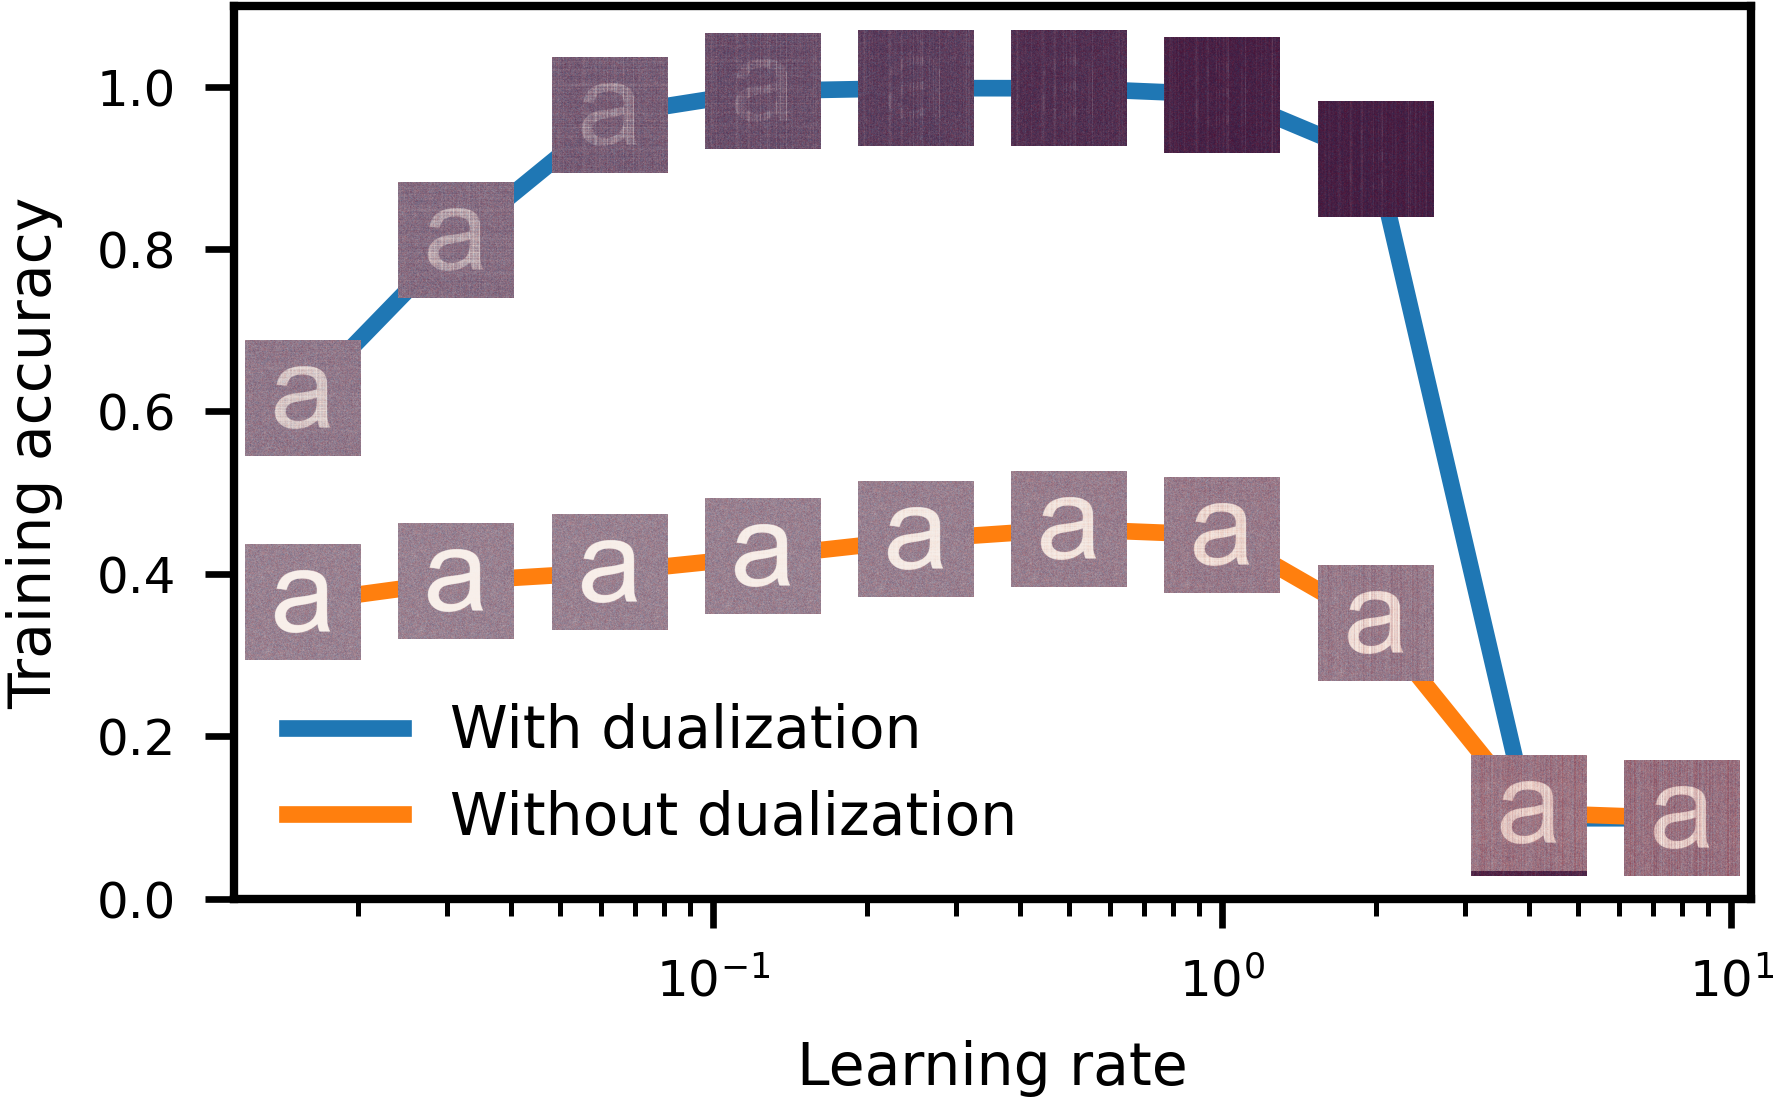
\includegraphics[width=0.85\linewidth]{figure/dualization/erasure.png}
    \caption{\textbf{Erasure of watermarked weights.} It is commonly held that the weights stay close to initialization in very wide networks \citep{NEURIPS2019_0d1a9651,math9182246}. To visualize the change in weights, we ``watermark'' the hidden layer weights of an MLP of width 1024 at initialization by zeroing out matrix entries in the shape of the letter ``a''. We then train for 1000 steps on CIFAR-10, across ten learning rates. For each run, we plot the final training accuracy along with an image of the learned weight matrix. Not only does dualized gradient descent reach higher training accuracies, but it also ``erases'' the watermark at the highest stable learning rate, a substantial weight change. More experimental details are available in Appendix A of ``Modular Duality in Deep Learning'' \citep{bernstein2024duality}.}
    \label{fig:weight-erasure}
\end{figure}